\section{The near field: mass seen through walls}\label{sec:near-field}

\begin{quote}
\textbf{In plain words.} The camera feels every nearby mass directly, through
anything in between, so it can see into a safe or weigh a lorry at a glance.
But the feeling blurs with distance, the way a hand under a thick blanket
shows only as a rough bump. Making the camera a million times more sensitive
makes the picture less than twice as sharp.
\end{quote}

In the near zone the camera measures the Newtonian tidal field of the scene as
it changes. Three properties follow at once. The field passes through all
matter, so no wall can screen a mass from the camera. Its strength is set by mass,
so the camera weighs what it sees. And it is present whether or not anything
moves, so a perfectly still scene is visible too.

\paragraph{How bright.} A body of mean density $\bar\rho$ and radius $R$ at
distance $r$ produces a tidal field of magnitude
\begin{equation}\label{eq:tidal-brightness}
\frac{2GM}{r^{3}} = \frac{8\pi G}{3}\,\bar\rho\,\theta^{3},
\qquad \theta = \frac{R}{r} .
\end{equation}
Tidal brightness is density times the cube of angular size. The Sun and the
Moon span the same angle in the sky, and the Moon, being denser, raises the
larger tide. A person one metre away spans a far larger angle than either,
and outweighs the Moon in the camera's view some fifty thousand times.

\paragraph{What the image is.} Summing Eq.~\eqref{eq:newton} over all the matter
in view, and grouping it by direction, gives the tidal field at the camera as
an integral over the sky,
\begin{equation}\label{eq:tidal-column}
\begin{gathered}
\tE_{ij} = G \int \dd\Omega\,\bigl(\delta_{ij} - 3\,\hat n_i \hat n_j\bigr)\,S(\hat n),\\
S(\hat n) = \int \rho(r\hat n)\,\frac{\dd r}{r} .
\end{gathered}
\end{equation}
The quantity $S$, which we call the \emph{tidal column}, is the mass along a
line of sight with each part weighted by the inverse of its distance;
Figure~\ref{fig:sky-integral} shows where the weighting comes from. The
integral starts a short distance $r_{\min}$ from the camera (a quarter of a
metre in the demonstrations), since matter at the camera itself would make $S$
diverge logarithmically, although not $\tE_{ij}$. A single pixel measures only
five numbers, the quadrupole of $S$ over the whole sky; an array, by comparing
the field from pixel to pixel, measures more.

\paragraph{What the image cannot show.} An array outside the matter it views
does not measure $S$ itself, because the field outside a body does not fix the
arrangement of mass inside it. A hollow shell and a solid ball of equal mass
produce the same field at every point outside both, however close. More
generally, adding to a body the density $\delta\rho = \nabla^2\chi/4\pi G$,
with $\chi$ any smooth function that vanishes outside it, changes the
potential by $\chi$ and so changes nothing outside \cite{YurtseverMarzbanMeila2011};
ordinary positive densities $\rho_0 \pm \epsilon\,\delta\rho$ make such pairs
out of real matter. The tidal column is therefore a rendering of a known
scene, the natural picture of what the camera responds to, and not a quantity
the camera could reconstruct uniquely. The near-field demonstrations show $S$
computed from the scene and blurred as described next. Other channels break
the ambiguity: the thermal glow shows a shell as a ring; a shell and a ball of
equal mass spinning at the same rate differ in $\tB_{ij}$ by the ratio of their
moments of inertia, $5/3$ (Section~\ref{sec:separation}), though at equal
angular momentum they are again alike; and a tide applied from outside probes
how the interior responds. The camera's position matters too: inside a closed
spherical shell it feels no tide from the shell at all, whatever its mass.

\begin{figure*}
\centering
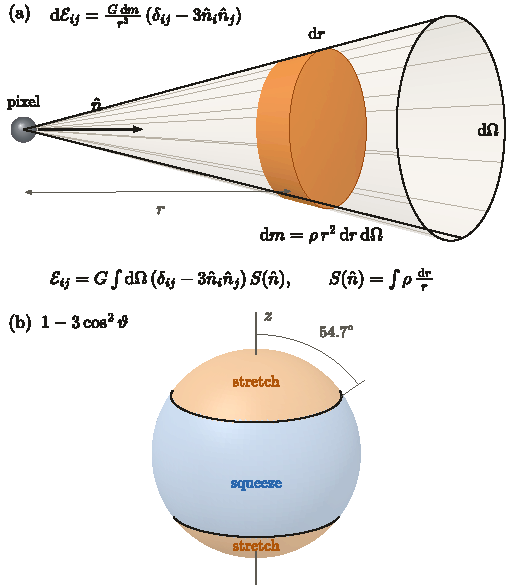
\includegraphics[width=\textwidth]{figures/sky-integral.pdf}
\caption{The sky integral, Eq.~\eqref{eq:tidal-column}. (a) A pixel at the apex
of a cone of directions $\dd\Omega$ about $\hat n$. The matter in the cone
between $r$ and $r + \dd r$, a piece of the cone bounded by two spherical caps
(orange), has mass $\dd m = \rho\,r^2\,\dd r\,\dd\Omega$ and adds
$G\,\dd m\,(\delta_{ij} - 3\hat n_i\hat n_j)/r^3$ to the tidal field. The $r^2$
of the volume cancels two of the three powers of $1/r$, so each line of sight
contributes its mass weighted by $\dd r/r$: the tidal column $S(\hat n)$. The
cone's width and $\dd r$ are exaggerated. (b) The sky around the pixel,
coloured by the sign of the weight $1 - 3\cos^2\vartheta$ with which one
component, $\tE_{zz}$, takes matter in each direction: matter in the orange caps,
within $54.7^\circ$ of the $z$ axis ($\cos^2\vartheta > 1/3$), stretches the
pixel along $z$; matter in the blue band squeezes it. The weight averages to
zero over the sky, which is why a uniform shell of matter around the camera is
invisible to it.}\label{fig:sky-integral}
\end{figure*}

\paragraph{What the image does show.} The ambiguity has an exact shape. For a
body whose outside is connected, every density splits in one way only into two
parts,
\begin{equation}\label{eq:split}
\rho = \rho_h + \frac{\nabla^2\chi}{4\pi G} ,
\end{equation}
where $\rho_h$ is harmonic inside the body, $\nabla^2\rho_h = 0$, and $\chi$
vanishes on the surface together with its gradient. The field outside fixes
$\rho_h$ completely and is blind to the rest \cite{Isakov1990}. The potential
outside is built from the moments $\int\rho\,h\,\dd V$ of the density against
functions $h$ harmonic in the body (the solid harmonics $r^\ell Y_{\ell m}$
about a point inside), and the second part has none of them, since
$\int h\,\nabla^2\chi\,\dd V = \int \chi\,\nabla^2 h\,\dd V = 0$. It follows that
any estimate of the interior that is linear in the data and treats every point
inside alike and independently, a white prior as in Eq.~\eqref{eq:wiener}, is
itself harmonic: it is built from the data's own kernels, which are. A harmonic
function has no maximum or minimum inside the region where it is harmonic. The
least assuming picture of an interior that a camera outside can draw, taking
the body's outline from light, therefore has its densest and its lightest
points on the surface. It can never show a core. Every round body appears as a
uniform ball of its mean density, and the layered Earth, seen from outside in
this way, as $5513\,\mathrm{kg\,m^{-3}}$ throughout.

Figure~\ref{fig:same-outside} shows three bodies with the same field outside. A
steel ball of radius $R$ holds a gold nugget of mass $m$ at the distance $s$
from its centre. The nugget's harmonic projection, the density harmonic in the
ball that has the same field outside, is
\begin{equation}\label{eq:harmonic-point}
\rho_h = \frac{m}{4\pi R^3}\sum_{\ell=0}^{\infty}(2\ell+1)(2\ell+3)\,
\Bigl(\frac{s r}{R^2}\Bigr)^{\ell} P_\ell(\cos\vartheta) ,
\end{equation}
with $\vartheta$ the angle from the nugget's direction; the sum has a closed
form, which the reference implementation uses. For $s = R/2$ it is a flush on
the wall nearest the nugget, $46\,m/4\pi R^3$ there, fifteen times the nugget's
mass spread evenly, fading toward the far wall, where it dips just below zero,
so that only the steel keeps it a real density. Poincar\'e's balayage sweeps the
same mass onto the surface as a skin of surface density
$m(R^2 - s^2)/4\pi R\,|\mathbf{x} - \mathbf{s}|^3$, thickest over the nugget. At
any sensitivity, a camera outside cannot tell the three apart.

\paragraph{What breaks the tie.} The three differ in one number that the
electric part cannot see, $\int\rho\,r^2\,\dd V$, the trace of the second
moment of the mass: $m s^2$, $\tfrac35\,m R^2$ and $m R^2$ for the nugget, the
flush and the skin ($r^2$ is not harmonic, so by Eq.~\eqref{eq:split} the
field outside carries no trace of it). The moment of inertia contains it,
$I_x = \tfrac23\int\rho\,r^2\,\dd V + \int\rho\,(r^2/3 - x^2)\,\dd V$, where the
second integral is harmonic and shared. Spun at the same rate about an axis
across the line to the nugget, the three therefore differ in angular momentum,
and so in the spin dipole of their magnetic fields
(Section~\ref{sec:separation}), by the gold's shares of the moment of inertia,
$0.25$, $0.48$ and $0.75\,mR^2$. The ball and the shell above, with
$\int\rho\,r^2\,\dd V = \tfrac35 MR^2$ and $MR^2$, are the simplest case. Spin
breaks only this one tie, since the moment of inertia is a single number. The
thermal glow, which sums along lines instead of reaching out as a potential,
would show the nugget as a spot, the flush as a gradient and the skin as a ring,
but the glow measures friction and temperature, not mass
(Section~\ref{sec:first-image}). A pixel inside the matter escapes the
ambiguity altogether, because there $\mathrm{tr}\,\tE = 4\pi G\rho$ reads the
density where the pixel is (Section~\ref{sec:pixel}).

Together the channels go further than any one. For the Earth the glow gives the
radius of the core, $3480\,\mathrm{km}$, from the kinks in its brightness
(Figure~\ref{fig:earth-inverted}); the electric part gives the mass; and the
magnetic part, with the rate of turning known, gives the moment of inertia,
$0.331\,MR^2$, the value the Preliminary Reference Earth Model is built to
match \cite{DziewonskiAnderson1981}. A two-layer Earth with that core, mass and
moment of inertia has a core of $12{,}500\,\mathrm{kg\,m^{-3}}$ and a mantle of
$4150\,\mathrm{kg\,m^{-3}}$. The reference model's core averages $10{,}900$; the
difference is the compression of the mantle under its own weight, which two
numbers cannot resolve.

\begin{figure}
\centering
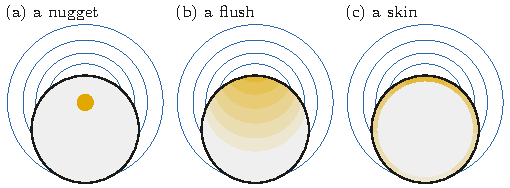
\includegraphics[width=\columnwidth]{figures/same-outside.pdf}
\caption{Same outside, different inside: three steel balls whose fields are
identical everywhere outside them. (a) A gold nugget halfway from the centre to
the wall. (b) Its harmonic projection, Eq.~\eqref{eq:harmonic-point}, the least
assuming interior that a camera outside could draw, shaded in bands that double
in density up to $46\,m/4\pi R^3$ at the near wall. (c) Its balayage: the
nugget's mass spread over the surface as a skin, drawn as a band of constant
width shaded in the same way, in steps that double in surface density up to
$6\,m/4\pi R^2$ over the nugget. Blue: equipotentials of the gold's share
of the field, drawn outside each ball (the steel's share is the same in all
three and is left out). They are the same in all three, and in (b) and (c) they
centre on a nugget that is not there. The reference implementation checks the
equality by integrating each body's potential directly.}\label{fig:same-outside}
\end{figure}

\paragraph{How sharp.} The space between scene and camera is empty, so the
potential there obeys Laplace's equation. Consider a pattern in the scene that
repeats across the line of sight with wavenumber $k$, at depth $z$ from the
sensor. Laplace's equation forces it to fade with height as
\begin{equation}\label{eq:evanescent}
\Phi \propto \cos(kx)\,e^{-kz} :
\end{equation}
fine detail dies away before it reaches the camera, and coarse detail
survives. To reconstruct the scene the camera must multiply each pattern by
$e^{kz}$, and its noise with it. If the largest features are recorded with
signal-to-noise ratio $\SNR$, patterns with $e^{kz} > \SNR$ are lost in the
noise, and detail finer than about $\pi z/\ln\SNR$ cannot be recovered.

The estimate can be made exact. Let a flat array at distance $z$ from a sheet
of sources with surface density $\sigma$ record the tidal field along its
normal with white noise of spectral density $N_0$. With $\Phi = -GM/r$ the
normal component above a mass is negative, a stretch, so we record
$d = -\tE_{zz}$. In Fourier space across the array the data are
\begin{equation}\label{eq:array-data}
\hat d(\mathbf k) = 2\pi G\,k\,e^{-kz}\,\hat\sigma(\mathbf k) + \hat n(\mathbf k),
\end{equation}
and the factor $k$ says that a uniform sheet is invisible: its pull is the
same at every pixel and at every height, so it has no tidal field at all.
Define the signal-to-noise ratio as the peak field of a
point mass $m$, $2Gm/z^3$, over the noise of the field averaged across a patch
of side $z$, $\sqrt{N_0}/z$: so $\SNR = 2Gm/(z^2\sqrt{N_0})$. Each Fourier
component of a point mass then stands above its own noise by
$s = \pi\,\SNR\;kz\,e^{-kz}$, and the best linear reconstruction (the Wiener
filter, which assumes the scene is a sheet of independent point masses) keeps
it with weight (taking as the prior a sheet of independent masses $m$, one
per area $z^2$, whose spectrum is $S_\sigma = m^2/z^2$)
\begin{equation}\label{eq:wiener}
H(k) = \frac{s^2}{1 + s^2}, \qquad s = \pi\,\SNR\;kz\,e^{-kz}.
\end{equation}
$H$ vanishes for a uniform scene, $k \to 0$, is close to one for patterns
between $kz \approx 1/\pi\SNR$ and $kz \approx 1$, and falls through one half
at $kz = q_c$, where
\begin{equation}\label{eq:cutoff}
q_c\,e^{-q_c} = \frac{1}{\pi\,\SNR},
\qquad
q_c \approx L + \ln L, \quad L = \ln(\pi\,\SNR)
\end{equation}
(10.1 against the exact 10.4 at $\SNR = 10^3$).
The image of a point is therefore close to the diffraction pattern of a round
pupil of radius $q_c/z$, $2J_1(x)/x$ with $x = q_c r/z$. The full width at half
maximum of this image, an amplitude and not its square, as an angle seen from
the array, is
\begin{equation}\label{eq:resolution}
\Delta\theta = \frac{4.43}{q_c}
\end{equation}
to within three per cent for every $\SNR \ge 100$ (for a single row of
sensors over a two-dimensional scene, $3.79/q_c$; the scene is then made of
line masses perpendicular to the row, and the potential obeys Laplace's
equation in two dimensions). Table~\ref{tab:resolution}
gives values, computed without approximation by the reference implementation
that accompanies the site, and Figure~\ref{fig:resolution-law} shows the law.

For an array at least as wide as the scene is deep, the angular blur does
not depend on distance or on the size of the array, only, through $q_c$, on the
logarithm of its sensitivity. A signal-to-noise ratio of a thousand gives
$24^\circ$; a million, $14^\circ$; $10^{30}$, still $3.4^\circ$. To match the
sharpness of the human eye, one arcminute, would take a signal-to-noise ratio
near $10^{6600}$. The first estimate $\pi/\ln\SNR$ is of the right size
everywhere, but it runs sharp at high sensitivity, because the image of a point
is wider than $\pi/q_c$. Figure~\ref{fig:nearfield} shows the reconstruction of
two masses, and the near-field demonstrations blur their images by
Eq.~\eqref{eq:resolution}. The same logarithmic limit is long familiar wherever
fields that obey Laplace's equation are continued back toward their sources: in
geophysics, where gravity and magnetic surveys are continued downward
\cite{Clarke1969,Parker1973}, and in near-field acoustic holography
\cite{MaynardWilliamsLee1985}.

\paragraph{A hand-held camera.} A camera much smaller than its distance from
the scene does worse. Inside a camera of width $D$, the part of the field that
varies over the sky with angular degree $\ell$ changes across the camera by a
factor $(D/2r)^{\ell-2}$ relative to the quadrupole, for a source at distance
$r$. Detail of degree $\ell$ therefore needs $\SNR \gtrsim (2r/D)^{\ell-2}$, and
\begin{equation}\label{eq:handheld}
\ell_{\max} \approx 2 + \frac{\ln\SNR}{\ln(2r/D)}, \qquad
\Delta\theta \approx \frac{\pi}{\ell_{\max}} .
\end{equation}
A camera ten centimetres across, looking at a lorry fifteen metres away with
$\SNR = 10^6$, sees detail of about $40^\circ$, not $14^\circ$. A single pixel,
$D \to 0$, sees the quadrupole alone. Widening the camera helps logarithmically
until it is about as wide as the scene is deep; beyond that,
Eq.~\eqref{eq:resolution} applies.

\paragraph{A blurred image is not a vague measurement.} The blur limits what
can be drawn of an arbitrary scene, not how precisely a simple one can be
measured. If the scene is known to hold a single point mass at depth $z$, an
infinite plane recording $\tE_{zz}$ with the noise above determines its
position to within $\sqrt{2/5}\,z/\mathcal{R}$ across and $z/\mathcal{R}$ in
depth, and its mass to within $\sqrt5/\mathcal{R}$ of itself, where
$\mathcal{R} = (\sqrt{3\pi}/4)\,\SNR$ is the signal-to-noise ratio of the whole
field pattern (the Cram\'er--Rao bounds with position and mass estimated
jointly, which we have checked by direct integration). At one metre and $\SNR = 10^3$ the mass is placed to within a
millimetre, while its image is $24^\circ$ wide. Two equal masses, by contrast,
can be told from one only when they are farther apart than about
$z/\sqrt{\mathcal{R}}$, because the difference they make grows as the square
of their separation. What limits the image is the variety of scenes allowed,
not the precision of the data.

\paragraph{How far can sensitivity go?} The premise of an arbitrarily sensitive
camera eventually meets the rest of physics. A heuristic argument, not a
theorem: a camera that fits within the distance $z$ to the scene, without
becoming a black hole, has a mass below $zc^2/2G$, so its energy of interaction
with a source of mass $M_s$ is below about $M_s c^2$. If quantum mechanics then
limits how quickly the camera's state can become distinguishable to a rate set
by that energy, as it does for a fixed coupling and a single measurement
task, over a time $\tau$ we would have $\SNR \lesssim M_s c^2\tau/\hbar$, with
$G$ and $z$ cancelling. For a person watched for the age of the universe this
is about $10^{70}$, a blur of $1.5^\circ$. On this estimate no near-field camera
could draw a face; making the estimate rigorous needs the coupling, the
resources and the discrimination task to be stated exactly.

\paragraph{How much a picture holds.} The resolution law says how fine the
detail of a near-field image can be. A different question, the one Shannon
asked of a telegraph line \cite{Shannon1948}, is how much the image can say:
how many bits the data carry about the scene. Equation~\eqref{eq:array-data}
answers it with no further assumption. Each Fourier component of the scene
reaches the array as a signal in additive Gaussian noise, standing above it by
the ratio $s$ of Eq.~\eqref{eq:wiener}, and components with different
$\mathbf k$ are independent. A real signal in Gaussian noise with power ratio
$s^2$ carries at most $\tfrac12\log_2(1+s^2)$ bits, a bound reached when the
signal is itself Gaussian, and a scene of area $A$ has $A\,\mathrm{d}^2k/(2\pi)^2$
real components in each $\mathrm{d}^2k$. Per area $z^2$ of the scene, with
$q = kz$, the data therefore hold
\begin{equation}\label{eq:capacity-integral}
C = \frac{1}{4\pi}\int_0^\infty q\,\log_2\!\left(1 + \pi^2\SNR^2 q^2 e^{-2q}\right)\mathrm{d}q
\end{equation}
bits about any scene with the spectrum of the prior of Eq.~\eqref{eq:wiener},
and a scene made of point masses carries somewhat less. Where $s > 1$, which
is for $q$ between about $1/\pi\SNR$ and $q_c$, the logarithm is close to
$2\log_2 s$; elsewhere it is small. Integrating $2q\log_2 s$ over that range,
with $\ln(\pi\SNR) = q_c - \ln q_c$ from Eq.~\eqref{eq:cutoff}, gives
\begin{equation}\label{eq:capacity}
C \approx \frac{q_c^3/3 - q_c^2/2}{4\pi\ln 2}
\end{equation}
to within three per cent for $\SNR \ge 10^3$ and half a per cent beyond
$10^{10}$.

The two terms have a plain reading. The patterns that survive the noise are
the components with $q < q_c$, and there are $q_c^2/4\pi$ of them per area
$z^2$; the rest of Eq.~\eqref{eq:capacity} is the number of bits each carries
on average, $(q_c/3 - \tfrac12)/\ln 2$, the mean of $2\log_2 s$ over them.
Greater sensitivity buys both more patterns and more bits in each, so with
$q_c \approx \ln\SNR$ the information grows, eventually, as
$(\ln\SNR)^3/12\pi\ln 2$: as the cube of the logarithm of the sensitivity. At
$\SNR = 10^3$ a near-field picture holds 38 bits per area $z^2$, about nine
patterns of four bits each. At $10^6$ it holds 200 bits; at $10^{30}$,
$1.6\times10^4$. At the heuristic ceiling of the previous paragraph, a person
watched for the age of the universe, it holds $1.8\times10^5$ bits, some 22
kilobytes, spread over 2{,}200 patterns of 80 bits each: about the size of a
thumbnail photograph, after sixty-seven orders of magnitude more sensitivity
(Figure~\ref{fig:capacity}). This is also why a blurred image and a precise
measurement are compatible. The data hold few bits, and a scene known to be
simple spends them all on a few numbers.

The camera's other channels scale differently, and the comparison shows what
is peculiar to the near field. A wave camera of width $D$ at wavelength
$\lambda$ resolves about $(D/\lambda)^2$ directions in each steradian, and each
carries about $\log_2\SNR$ bits: the aperture fixes the number of patterns, and
sensitivity adds bits only in proportion to its logarithm. In the near field
there is no aperture to fix the number of patterns; sensitivity sets it
through $e^{-kz}$, and that is why the power is three rather than one. A single
pixel, at the other extreme, is limited by geometry rather than noise: from a
sky of many overlapping sources it learns twenty-five numbers however
sensitive it is (Section~\ref{sec:no-lens}). And the thermal glow, recorded by
counting gravitons, is limited by their number: $N$ gravitons over $M$
resolution cells carry at most about $N\log_2 M$ bits. A camera a metre square
looking down at the Earth for a year counts about 1{,}750 of them in the model
of Section~\ref{sec:first-image}, so its picture of the planet's interior holds
a few kilobytes at any reasonable resolution.

\begin{table}
\centering
\begin{tabular}{rrrrrr}
$\SNR$ & $q_c$ & array & row & two points & $\pi/\ln\SNR$ \\ \hline
$10^{3}$ & 10.4 & 24.0° & 20.7° & 24.5° & 26.1° \\
$10^{6}$ & 17.8 & 14.1° & 12.1° & 14.6° & 13.0° \\
$10^{10}$ & 27.5 & 9.2° & 7.9° & 9.5° & 7.8° \\
$10^{20}$ & 51.1 & 5.0° & 4.2° & 5.1° & 3.9° \\
$10^{30}$ & 74.5 & 3.4° & 2.9° & 3.5° & 2.6° \\
$10^{60}$ & 144.3 & 1.8° & 1.5° & 1.8° & 1.3° \\
\end{tabular}
\caption{Blur of the near-field image. ``Array'': full width at half maximum
of the reconstructed image of a point, for a flat array, Eq.~\eqref{eq:resolution}.
``Row'': the same for a single row of sensors over a two-dimensional scene.
``Two points'': the smallest separation at which two equal point masses show
a dip between them in the array's image (Sparrow's criterion); because the
Wiener filter rolls off gradually, this slightly exceeds the full width, the
reverse of a sharp-edged pupil. The last column is the first estimate.}\label{tab:resolution}
\end{table}

\begin{figure*}
\centering
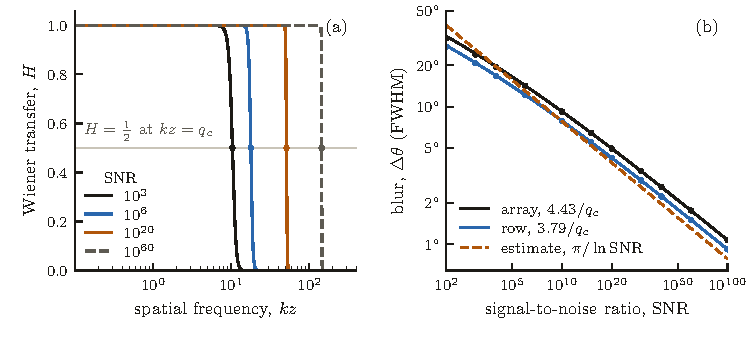
\includegraphics[width=\textwidth]{figures/resolution-law.pdf}
\caption{The exact near-field resolution law. (a) The Wiener filter $H$ of
Eq.~\eqref{eq:wiener} against spatial frequency, for four signal-to-noise
ratios: patterns coarser than $kz = q_c$ are kept almost whole, finer ones are
lost. Dots mark $H = \tfrac12$ at $q_c$, Eq.~\eqref{eq:cutoff}. Raising the
sensitivity from $10^{6}$ to $10^{60}$ moves the cutoff only from 18 to 144.
(b) The resulting blur, the full width at half maximum of the image of a
point, for a flat array ($4.43/q_c$) and a single row ($3.79/q_c$), with
values computed directly by the reference implementation (dots) and the first
estimate $\pi/\ln\SNR$ (dashed).}\label{fig:resolution-law}
\end{figure*}

\begin{figure}
\centering
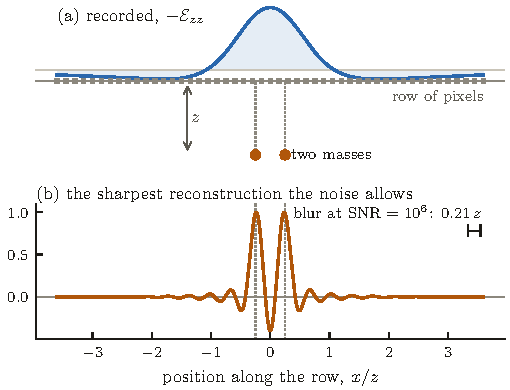
\includegraphics[width=\columnwidth]{figures/nearfield.pdf}
\caption{The near-field blur, for a row of pixels over a
two-dimensional scene: two line masses a distance $z/2$ apart at depth $z$, recorded
with signal-to-noise ratio $10^6$. (a) The geometry, to scale, and what the
pixels record: $\tE_{zz}$ along the row, a single smooth bump. (b) The best
reconstruction of the masses that the noise allows, the Wiener filter of
Eq.~\eqref{eq:wiener}, computed by the reference implementation; its ripples
are the price of discarding the detail that noise has swamped. The bar is the
blur, $0.21\,z$. On the website the sensitivity and the separation can be
changed.}\label{fig:nearfield}
\end{figure}

\begin{figure}
\centering
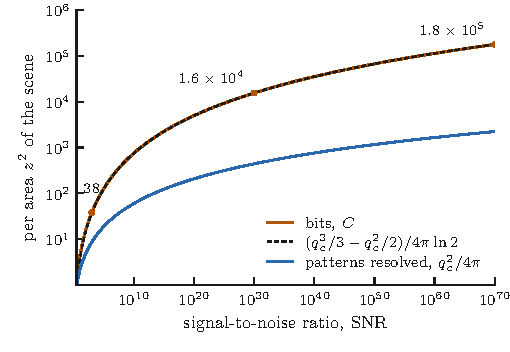
\includegraphics[width=\columnwidth]{figures/capacity.pdf}
\caption{How much a near-field picture holds, per area $z^2$ of the scene,
against the signal-to-noise ratio. Orange: the bits the data carry about the
scene, Eq.~\eqref{eq:capacity-integral}, computed by the reference
implementation. Dashed: the closed form of Eq.~\eqref{eq:capacity}, which lies
on it. Blue: the number of independent patterns resolved, $q_c^2/4\pi$. Raising
the sensitivity by sixty-seven orders of magnitude, from $10^3$ to $10^{70}$,
raises the information only from 38 bits to $1.8\times10^5$, about 22
kilobytes.}\label{fig:capacity}
\end{figure}

The logarithmic limit is the central result for the whole subject. The near field
is where everyday things are visible, and it can never be sharp. Sharp images
need waves.

\begin{figure*}
\centering
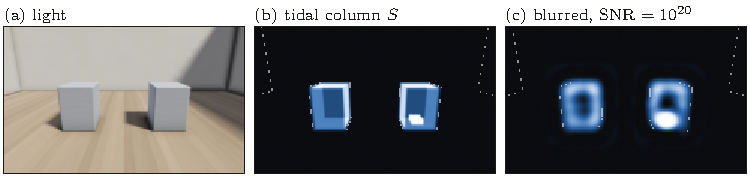
\includegraphics[width=\textwidth]{figures/locked-safe.pdf}
\caption{The locked safe, computed. Two identical steel safes
$3.5\,\mathrm{m}$ away; the right-hand one holds $320\,\mathrm{kg}$ of gold.
(a) Ordinary light, from the same camera. (b) The tidal column $S(\hat n)$ of
Eq.~\eqref{eq:tidal-column}, exact, with the empty room left out; white lines
mark the outlines that light shows. (c) The same, blurred by the point spread
of the Wiener reconstruction at a signal-to-noise ratio of $10^{20}$,
Eq.~\eqref{eq:resolution}: the gold still stands out through the steel.
Blurring $S$ in this way treats the scene as if it lay at a single depth; it
shows what an array as wide as the scene is deep could resolve, not a
reconstruction from simulated data (Section~\ref{sec:near-field}).}\label{fig:locked-safe}
\end{figure*}
